\documentclass[12pt]{article}

\usepackage[T1]{fontenc}
\usepackage{mathptmx}
\usepackage[margin=1in]{geometry}
\usepackage{amsmath, amssymb}
\usepackage{graphicx}
\usepackage{booktabs}
\usepackage{threeparttable}
\usepackage{authblk}
\usepackage{hyperref}
\usepackage{xcolor}
\usepackage{listings}
\hypersetup{colorlinks=true, linkcolor=blue, citecolor=blue, urlcolor=blue}

\lstset{
  basicstyle=\ttfamily\footnotesize,
  breaklines=true,
  frame=single,
  columns=fullflexible
}

\title{Cognitive Bandwidth and Administrative Friction in Household Debt:\\
A Structurally Estimated Model Calibrated to the\\
2025 Survey of Household Economics and Decisionmaking}
\author{Eithan Alexander Valenzuela}
\affil{Independent Research}
\date{\today}

\begin{document}
\maketitle

\begin{abstract}
\noindent A recurring claim in behavioral public finance is that low-income households are held back from beneficial financial actions not only by insufficient liquidity but by the ``administrative sludge'' of formal channels: the paperwork, time, and attention that refinancing, disputing, or applying for credit require. This paper builds a small structural model in which a household's monthly financial choice is jointly constrained by a budget constraint (feasibility) and a depletable cognitive bandwidth (accessibility), and estimates the model's key behavioral parameters by the Simulated Method of Moments (SMM) against three real, cited statistics from the Federal Reserve Board's 2025 Survey of Household Economics and Decisionmaking (SHED, $n=12{,}934$). We document a specific, falsifiable methodological finding along the way: fixing the monthly income-shock arrival probability at a plausible-looking assumed value (4\%) makes the model unable to reconcile simulated payday-loan incidence with the real SHED rate no matter how the behavioral parameters are tuned (residual sum of squared errors plateaus near $0.02$); treating the shock arrival probability itself as an estimated parameter resolves this, dropping the fit residual by roughly two orders of magnitude. Using the resulting exactly-identified, three-parameter calibration, we simulate a paired, common-random-numbers counterfactual comparing a one-time \$500 cash transfer, a reduction in the cognitive cost of formal refinancing (``sludge eradication''), and both together, against a no-intervention control, on a synthetic population of 4,000 households replayed under four policy regimes. We do \emph{not} find evidence that the two interventions are complementary: the estimated interaction effect is small and its 95\% paired-bootstrap confidence interval, $[-0.0010, +0.0005]$, comfortably includes zero. We report this null result as the paper's central, defensible finding, alongside a candid discussion of why it may partly reflect the fixed timing of the simulated cash transfer rather than a definitive absence of complementarity, and of several other disclosed limitations of the calibration.

\vspace{0.5cm}
\noindent \textbf{JEL Codes:} D14, D91, D18, I38 \\
\textbf{Keywords:} Household Finance, Cognitive Bandwidth, Administrative Sludge, Simulated Method of Moments, Survey of Household Economics and Decisionmaking
\end{abstract}

\newpage
\tableofcontents
\newpage

\section{Introduction}

Two traditions in household finance offer competing explanations for why some households persistently rely on high-cost credit even when, on paper, a cheaper alternative is available. The neoclassical tradition emphasizes \emph{feasibility}: households use payday loans, pawn loans, or carry a revolving credit-card balance because they lack the liquidity to do otherwise, full stop. A newer behavioral tradition, associated with the psychology-of-scarcity literature \cite{mullainathan2013scarcity} and the public-administration literature on ``sludge'' \cite{sunstein2019sludge, bhargava2015psychological}, argues that \emph{accessibility} is a second, independent constraint: even a household with enough money to refinance a debt, dispute a fee, or apply for a formal loan may fail to do so because the administrative burden of the formal channel exceeds what a financially stressed mind has left to give it.

This paper takes that second claim seriously enough to build a model in which it can fail. We specify a monthly household decision problem with two constraints operating side by side: a standard budget constraint, and a cognitive-bandwidth constraint that shrinks under financial stress and gates which of the household's otherwise-affordable options it can actually execute. We then do something the existing behavioral literature on sludge, to our knowledge, has not combined in one place: we structurally estimate the model's key behavioral parameters against real, government-collected microdata using the Simulated Method of Moments (SMM), and we use the fitted model to run a counterfactual policy comparison between a cash-based intervention (which relaxes the budget constraint) and a friction-reducing intervention (which relaxes the bandwidth constraint), testing directly whether the two are complements.

The paper is deliberately narrow in scope and honest about it. We do not claim to have identified the true structural parameters of the American household sector; a two-or-three-parameter model fit to two or three moments is a diagnostic instrument, not a census. What we do claim, and defend with a fully reproducible pipeline, is: (i) a specific and useful methodological finding about when a plausible-looking modeling assumption quietly makes a calibration exercise impossible to fit, discovered and resolved in the course of this project; and (ii) a specific, real, and — as far as this model and this vintage of data can tell us — \emph{null} finding about the complementarity of cash and friction-reduction as household-debt policy levers, which we report as a legitimate result rather than a disappointment.

The rest of the paper is organized as follows. Section 2 reviews the relevant literature. Section 3 presents the structural model. Section 4 describes the data. Section 5 describes the SMM estimation strategy, including the discovery that motivated freeing the shock-arrival parameter. Section 6 reports the fitted parameters and the model's fit to the real target moments. Section 7 reports the policy counterfactual and the central null finding. Section 8 discusses robustness, limitations, and what would need to change to strengthen or overturn the finding. Section 9 concludes.

\section{Related Literature}

This paper sits at the intersection of three literatures. First, the psychology of scarcity \cite{mullainathan2013scarcity} argues that operating under severe financial constraint imposes a direct tax on cognitive bandwidth — attention, working memory, and impulse control all degrade under scarcity in a way that is separable from, and compounds, the scarcity itself. Second, the public-administration literature on ``sludge'' \cite{sunstein2019sludge} formalizes the idea that friction in accessing a beneficial program or product is not a neutral inconvenience but a policy-relevant variable in its own right; \cite{bhargava2015psychological} provide a well-identified empirical demonstration of exactly this mechanism in a large-scale IRS field experiment on incomplete take-up of a tax benefit. Third, the empirical literature on high-cost consumer credit — most directly \cite{melzer2011real} on the real costs of payday-loan access and \cite{skiba2019payday} on payday loans and bankruptcy — establishes both that access to predatory credit has measurable welfare consequences and that households who use it are not obviously irrational; they are frequently making a constrained choice among worse options.

Our contribution relative to this literature is narrow but specific: we translate the qualitative claim that ``bandwidth and budget are separate constraints'' into a model in which that claim has testable, quantitative content, and we discipline the model's free parameters with real survey data rather than choosing them by introspection. The estimation approach follows the Simulated Method of Moments tradition of \cite{mcfadden1989method}: when a model's likelihood is intractable or the model is more naturally specified as a simulator than as a closed-form density, one instead matches simulated moments to empirical ones by numerical search. We are not aware of prior work that combines a bandwidth/sludge behavioral model with SMM estimation against the SHED specifically, which is what this paper's methodological contribution consists of.

\section{The Structural Model}

\subsection{Household state and cognitive bandwidth}

A household $i$ is characterized in month $t$ by a liquid balance $B_{i,t}$, a revolving-debt balance $D_{i,t}$, a payday-debt balance $P_{i,t}$, monthly income $Y_{i,t}$, fixed monthly obligations $O_i$, and a cognitive bandwidth $\Omega_{i,t} \in [a_{\min}, 1]$. Bandwidth evolves as a stress-driven exponential moving average:
\begin{equation}
    \Omega_{i,t} = \max\left(a_{\min},\ (1-\rho)\,\Omega_{i,t-1} + \rho \cdot \max\!\left(a_{\min},\ 1 - \alpha \cdot s_{i,t}\right)\right)
\end{equation}
where $\rho \in (0,1]$ is an assumed adjustment speed, $\alpha$ is the paper's central estimated \emph{stress elasticity}, and $s_{i,t}$ is a stress ratio capturing how tightly obligations and required debt payments are stretched against available resources that month, capped at $s_{\max}=3$:
\begin{equation}
    s_{i,t} = \min\left(s_{\max},\ \frac{O_i + R_{i,t}}{\max(B_{i,t} + Y_{i,t},\ 1)}\right)
\end{equation}
with $R_{i,t}$ the sum of the required minimum payments on revolving and payday debt that month.

\subsection{The bifurcated choice set}

Each month, resources available for debt service are $X_{i,t} = B_{i,t} + Y_{i,t} - O_i$, and the household selects one of four actions: pay the minimum ($\texttt{PAY\_MIN}$), formally refinance ($\texttt{REFI}$), defer/partially pay ($\texttt{DEFER}$), or take a payday loan ($\texttt{PAYDAY}$). Each action $j$ has a \emph{feasibility} condition (can the household afford it) and a \emph{cognitive cost} $c_j \in [0,1]$ (can the household's current bandwidth reach it):

\begin{align}
    \text{PAY\_MIN feasible} &\iff X_{i,t} \ge R_{i,t} \\
    \text{REFI feasible} &\iff \text{offer available} \wedge \text{not already refinanced} \wedge X_{i,t} \ge R_{i,t} + \text{refi fee} \\
    \text{DEFER feasible} &\iff 0 \le X_{i,t} < R_{i,t} \\
    \text{PAYDAY feasible} &\iff X_{i,t} < R_{i,t}
\end{align}

An action is \emph{accessible} if it is feasible \emph{and} $c_j \le \Omega_{i,t}$. If the feasible set is nonempty but the accessible set is empty — the household can afford something but its bandwidth has fallen below every option's cognitive cost — we record a \emph{cognitive collapse}, financially equivalent to a forced payday loan. This is the model's formal device for the sludge hypothesis: it is possible, by construction, for a household to be denied an action not because it cannot afford it but because it cannot presently execute it.

Among the accessible actions, the household picks the one minimizing an expected long-run cost $\kappa_j$ (fees plus the present value of future interest under a fixed horizon $H=12$ months), with $\texttt{PAY\_MIN}$ normalized to $\kappa=0$:
\begin{equation}
    \kappa_{\texttt{REFI}} = \text{fee} - H\cdot\bar D_{i,t}\cdot(r_{\text{high}}-r_{\text{low}}), \quad
    \kappa_{\texttt{DEFER}} = \text{fee} + H\cdot r_{\text{high}}\cdot R^{\text{formal}}_{i,t}, \quad
    \kappa_{\texttt{PAYDAY}} = \ell\cdot(\text{fee}+r_{\text{pd}} H) + g\cdot(\text{late fee}+r_{\text{high}}H)
\end{equation}
where $\ell$ and $g$ split any shortfall between what a capped payday loan can cover and an uncovered gap. All interest rates, fees, and cognitive-cost \emph{levels} in this specification are assumed, not estimated, and are disclosed as such directly in the project's source code (\texttt{src/model/params.py}); only $\alpha$, $c_{\texttt{payday}}$, and the exogenous shock-arrival probability described in Section 5 are estimated from data.

\section{Data}

\subsection{Source}

Target moments are drawn from the Board of Governors of the Federal Reserve System's 2025 Survey of Household Economics and Decisionmaking (SHED), the thirteenth wave of an annual survey of U.S. adults conducted online by Ipsos on its probability-based KnowledgePanel. The 2025 wave was fielded in October 2025 and the accompanying report and public-use codebook were released May 13, 2026 ($n=12{,}934$).\footnote{Codebook: \url{https://www.federalreserve.gov/consumerscommunities/files/SHED_2025codebook.pdf}. Public-use microdata (not used directly in this paper's headline estimates; see Section 8.1): \url{https://www.federalreserve.gov/consumerscommunities/files/SHED_public_use_data_2025_(CSV).zip}.}

\subsection{Target moments}

We use three published, unweighted response counts directly from the codebook, chosen because each maps onto a specific model construct without requiring the raw microdata file (Table \ref{tab:moments}).

\begin{table}[h]
\centering
\begin{threeparttable}
\begin{tabular}{@{}llrrr@{}}
\toprule
\textbf{Model moment} & \textbf{SHED variable} & \textbf{Count} & \textbf{$n$} & \textbf{Share} \\
\midrule
$m_1$: payday capture (12mo) & \texttt{BK2\_c} & 501 & 12,934 & 3.87\% \\
$m_2$: chronic revolver share & \texttt{C4A} = 3 & 2,320 & 10,759\tnote{a} & 21.56\% \\
$m_3$: missed min. payment (last mo.) & \texttt{C3P} = 2 & 284 & 10,120\tnote{b} & 2.81\% \\
\bottomrule
\end{tabular}
\begin{tablenotes}
\small
\item[a] Denominator restricted to respondents holding at least one credit card (\texttt{C2A}=Yes).
\item[b] Denominator restricted to cardholders who carried any balance last month (excludes \texttt{C3P}=$-9$, ``no balance'').
\end{tablenotes}
\end{threeparttable}
\caption{Real target moments and their exact source. Counts and question wording verified directly against the published 2025 SHED codebook.}
\label{tab:moments}
\end{table}

$\texttt{BK2\_c}$ asks whether the respondent or their spouse/partner took out a payday loan or payday advance in the past 12 months, mapping directly onto the model's $\texttt{PAYDAY}$/collapse capture event. $\texttt{C4A}$ asks cardholders how frequently they carried an unpaid balance over the past 12 months; we use the ``most or all of the time'' category as the model's chronic-revolver analog. $\texttt{C3P}$ asks specifically about last month, giving an approximate (not exact) analog to the model's $\texttt{DEFER}$ action, disclosed as a limitation in Section 8.2.

\subsection{A disclosed data limitation: unweighted counts}

The counts in Table \ref{tab:moments} are unweighted response frequencies as tabulated directly in the codebook, not the survey-weighted population estimates the Federal Reserve itself reports in the accompanying ``Economic Well-Being of U.S. Households'' publication. SHED's public-use file includes a post-stratification weight (\texttt{weight}) for exactly this purpose. We did not have the raw microdata file available in the computing environment used to write this paper (see Section 8.1 for why), so we could not compute $\sum w_i \mathbb{1}[\cdot] / \sum w_i$ directly. We flag this explicitly rather than presenting the unweighted counts as population-representative; Section 8.1 gives the exact steps needed to redo the calibration with weighted moments once the raw file is available.

\section{Estimation Strategy}

\subsection{Simulated Method of Moments with Common Random Numbers}

Let $\theta$ collect the model's estimated parameters and $\hat M(\theta)$ the vector of simulated moments produced by running the model on a fixed synthetic population under candidate $\theta$. The SMM estimator solves
\begin{equation}
    \hat\theta = \arg\min_\theta \ \lVert M - \hat M(\theta) \rVert_2^2
\end{equation}
where $M$ is the vector of real target moments from Table \ref{tab:moments}. Because $\hat M(\theta)$ is produced by a stochastic simulation, a naive implementation re-draws random shocks on every evaluation of the objective, producing a noisy, non-smooth surface on which standard optimizers behave erratically. We instead fix every household's underlying random draws (income shocks, refinance-offer timing) once, before optimization begins, and reuse them unchanged across every $\theta$ the optimizer tries — the standard Common Random Numbers (CRN) technique. We verify this is implemented correctly with an explicit repeated-call determinism test (\texttt{tests/test\_invariants.py}, and see Appendix~B) and use a global, derivative-free optimizer (differential evolution) appropriate to the resulting deterministic-but-non-smooth objective surface.

\subsection{A methodological discovery: why the shock-arrival rate had to be estimated, not assumed}

Our first specification fixed the monthly probability that a household begins a new income-shock spell, $p_{\text{start}}$, at an assumed value of 4\%, treating only $(\alpha, c_{\texttt{payday}})$ as estimated against the two moments $(m_1, m_2)$. This is a natural first modeling choice: shock frequency is not the paper's behavioral quantity of interest, so it is tempting to fix it at a plausible-looking value and estimate around it. Running the two-parameter estimator this way converged to $\hat\alpha = 1.5622$, $\hat c_{\texttt{payday}} = 0.5984$, with a residual sum of squared errors of $0.019956$ — small in absolute terms, but almost entirely attributable to a single moment: the model matched $m_2$ almost exactly (target $0.2156$, fitted $0.2160$) while overshooting $m_1$ by more than four-fold (target $0.0387$, fitted $0.1800$).

To diagnose whether this was a genuine model misspecification or simply an unlucky optimizer run, we re-estimated $(\alpha, c_{\texttt{payday}})$ at several \emph{fixed} values of $p_{\text{start}}$ and tracked the best achievable fit at each (Table \ref{tab:pstart_diagnostic}).

\begin{table}[h]
\centering
\begin{tabular}{@{}lrrr@{}}
\toprule
$p_{\text{start}}$ (fixed) & $\hat\alpha$ & $\hat c_{\texttt{payday}}$ & SSE \\
\midrule
0.005 & 1.291 & 0.699 & 0.00050 \\
0.010 & 1.544 & 0.686 & 0.00034 \\
0.020 & 1.424 & 0.684 & 0.00329 \\
0.040 & 0.843 & 0.597 & 0.01996 \\
\bottomrule
\end{tabular}
\caption{Best two-parameter fit against real moments $(m_1,m_2)$ at several fixed shock-arrival rates. Fit improves by roughly two orders of magnitude between the originally assumed rate (4\%) and roughly 1\%.}
\label{tab:pstart_diagnostic}
\end{table}

The pattern is unambiguous: the assumed 4\% monthly shock rate is simply too high to be consistent with the real 12-month payday-loan incidence rate, regardless of how the behavioral parameters are tuned. This is exactly the situation in which an assumed nuisance parameter is silently doing load-bearing work in a calibration exercise. The methodologically correct response is not to hand-pick a better-looking fixed value, but to make the shock-arrival rate itself an estimated parameter and add a third real target moment so the resulting system remains identified.

\subsection{Final specification: three parameters, three moments, exactly identified}

The paper's final specification estimates $\theta = (\alpha,\ c_{\texttt{payday}},\ p_{\text{start}})$ against the three moments in Table \ref{tab:moments} — three free parameters, three target moments, exactly identified in the classical method-of-moments sense. $m_3$ is operationalized in the simulation as the share of all household-months (not just shortfall months) resolved by the $\texttt{DEFER}$ action, an approximation to $\texttt{C3P}$'s ``last month'' framing whose quality we assess directly in Section 8.2.

\subsection{Estimator validation against a known synthetic ground truth}

Before trusting any estimate from real data, we validate the three-parameter estimator against a synthetic ground truth: we simulate a population under a known, hidden $\theta_{\text{true}} = (0.55,\ 0.20,\ 0.02)$, treat its resulting moments as if they were the ``real'' target, and check whether an estimator that never sees $\theta_{\text{true}}$ can recover it. The estimator matches the target moments closely (SSE $= 0.00005$; Table~\ref{tab:validation}), and its point estimate for the shock-arrival parameter in particular is close to the truth ($\hat p_{\text{start}}=0.0178$ vs.\ true $0.02$), which is reassuring given that parameter is the paper's central diagnostic discovery. The recovered $\hat\alpha$ and $\hat c_{\texttt{payday}}$ are farther from their true values despite the low SSE — a genuine identification-strength issue we return to in Section 8.3, not swept under the rug.

\begin{table}[h]
\centering
\begin{tabular}{@{}lrrr@{}}
\toprule
& $\alpha$ & $c_{\texttt{payday}}$ & $p_{\text{start}}$ \\
\midrule
True (hidden) & 0.5500 & 0.2000 & 0.0200 \\
Recovered & 0.2814 & 0.4357 & 0.0178 \\
Bootstrap mean ($B=20$) & 1.0004 & 0.4396 & 0.0201 \\
Bootstrap SE & 0.5677 & 0.0885 & 0.0057 \\
\bottomrule
\end{tabular}
\caption{Ground-truth recovery check. Target moments matched at SSE $=0.00005$.}
\label{tab:validation}
\end{table}

\section{Estimation Results}

Running the exactly-identified, three-parameter estimator against the three real SHED moments in Table \ref{tab:moments} yields
\begin{equation}
    \hat\alpha = 1.3345, \qquad \hat c_{\texttt{payday}} = 0.6929, \qquad \hat p_{\text{start}} = 0.0076,
\end{equation}
with a final SSE of $0.000763$ — roughly 26 times smaller than the best two-parameter fit at any fixed shock rate we tried in Table \ref{tab:pstart_diagnostic}, and roughly 26,000 times smaller than the original assumed-shock-rate specification. Table \ref{tab:fit} reports the fit to each individual moment.

\begin{table}[h]
\centering
\begin{tabular}{@{}lrrr@{}}
\toprule
Moment & Target & Fitted & Abs. error \\
\midrule
$m_1$ (payday, 12mo) & 0.0387 & 0.0440 & 0.0053 \\
$m_2$ (chronic revolver) & 0.2156 & 0.2174 & 0.0018 \\
$m_3$ (deferred payment) & 0.0281 & 0.0010 & 0.0271 \\
\bottomrule
\end{tabular}
\caption{Fit at the final three-parameter estimate.}
\label{tab:fit}
\end{table}

$m_1$ and $m_2$ are matched closely. $m_3$ is not: the model substantially underpredicts real-world use of partial/deferred payment. We discuss why in Section 8.2 rather than treat the aggregate SSE improvement as license to ignore a moment-specific shortfall.

Bootstrap standard errors ($B=20$ resamples of the estimation population, with replacement, full re-estimation each time) are reported in Table \ref{tab:bootstrap_real}.

\begin{table}[h]
\centering
\begin{tabular}{@{}lrr@{}}
\toprule
Parameter & Bootstrap mean & Bootstrap SE \\
\midrule
$\alpha$ & 0.9811 & 0.4918 \\
$c_{\texttt{payday}}$ & 0.6906 & 0.0668 \\
$p_{\text{start}}$ & 0.0095 & 0.0050 \\
\bottomrule
\end{tabular}
\caption{Bootstrap standard errors, real-data calibration.}
\label{tab:bootstrap_real}
\end{table}

The stress elasticity $\alpha$ carries a wide bootstrap SE relative to its point estimate — a genuine weak-identification finding discussed in Section 8.3, not a number to be quoted without its uncertainty.

\begin{figure}[h]
\centering
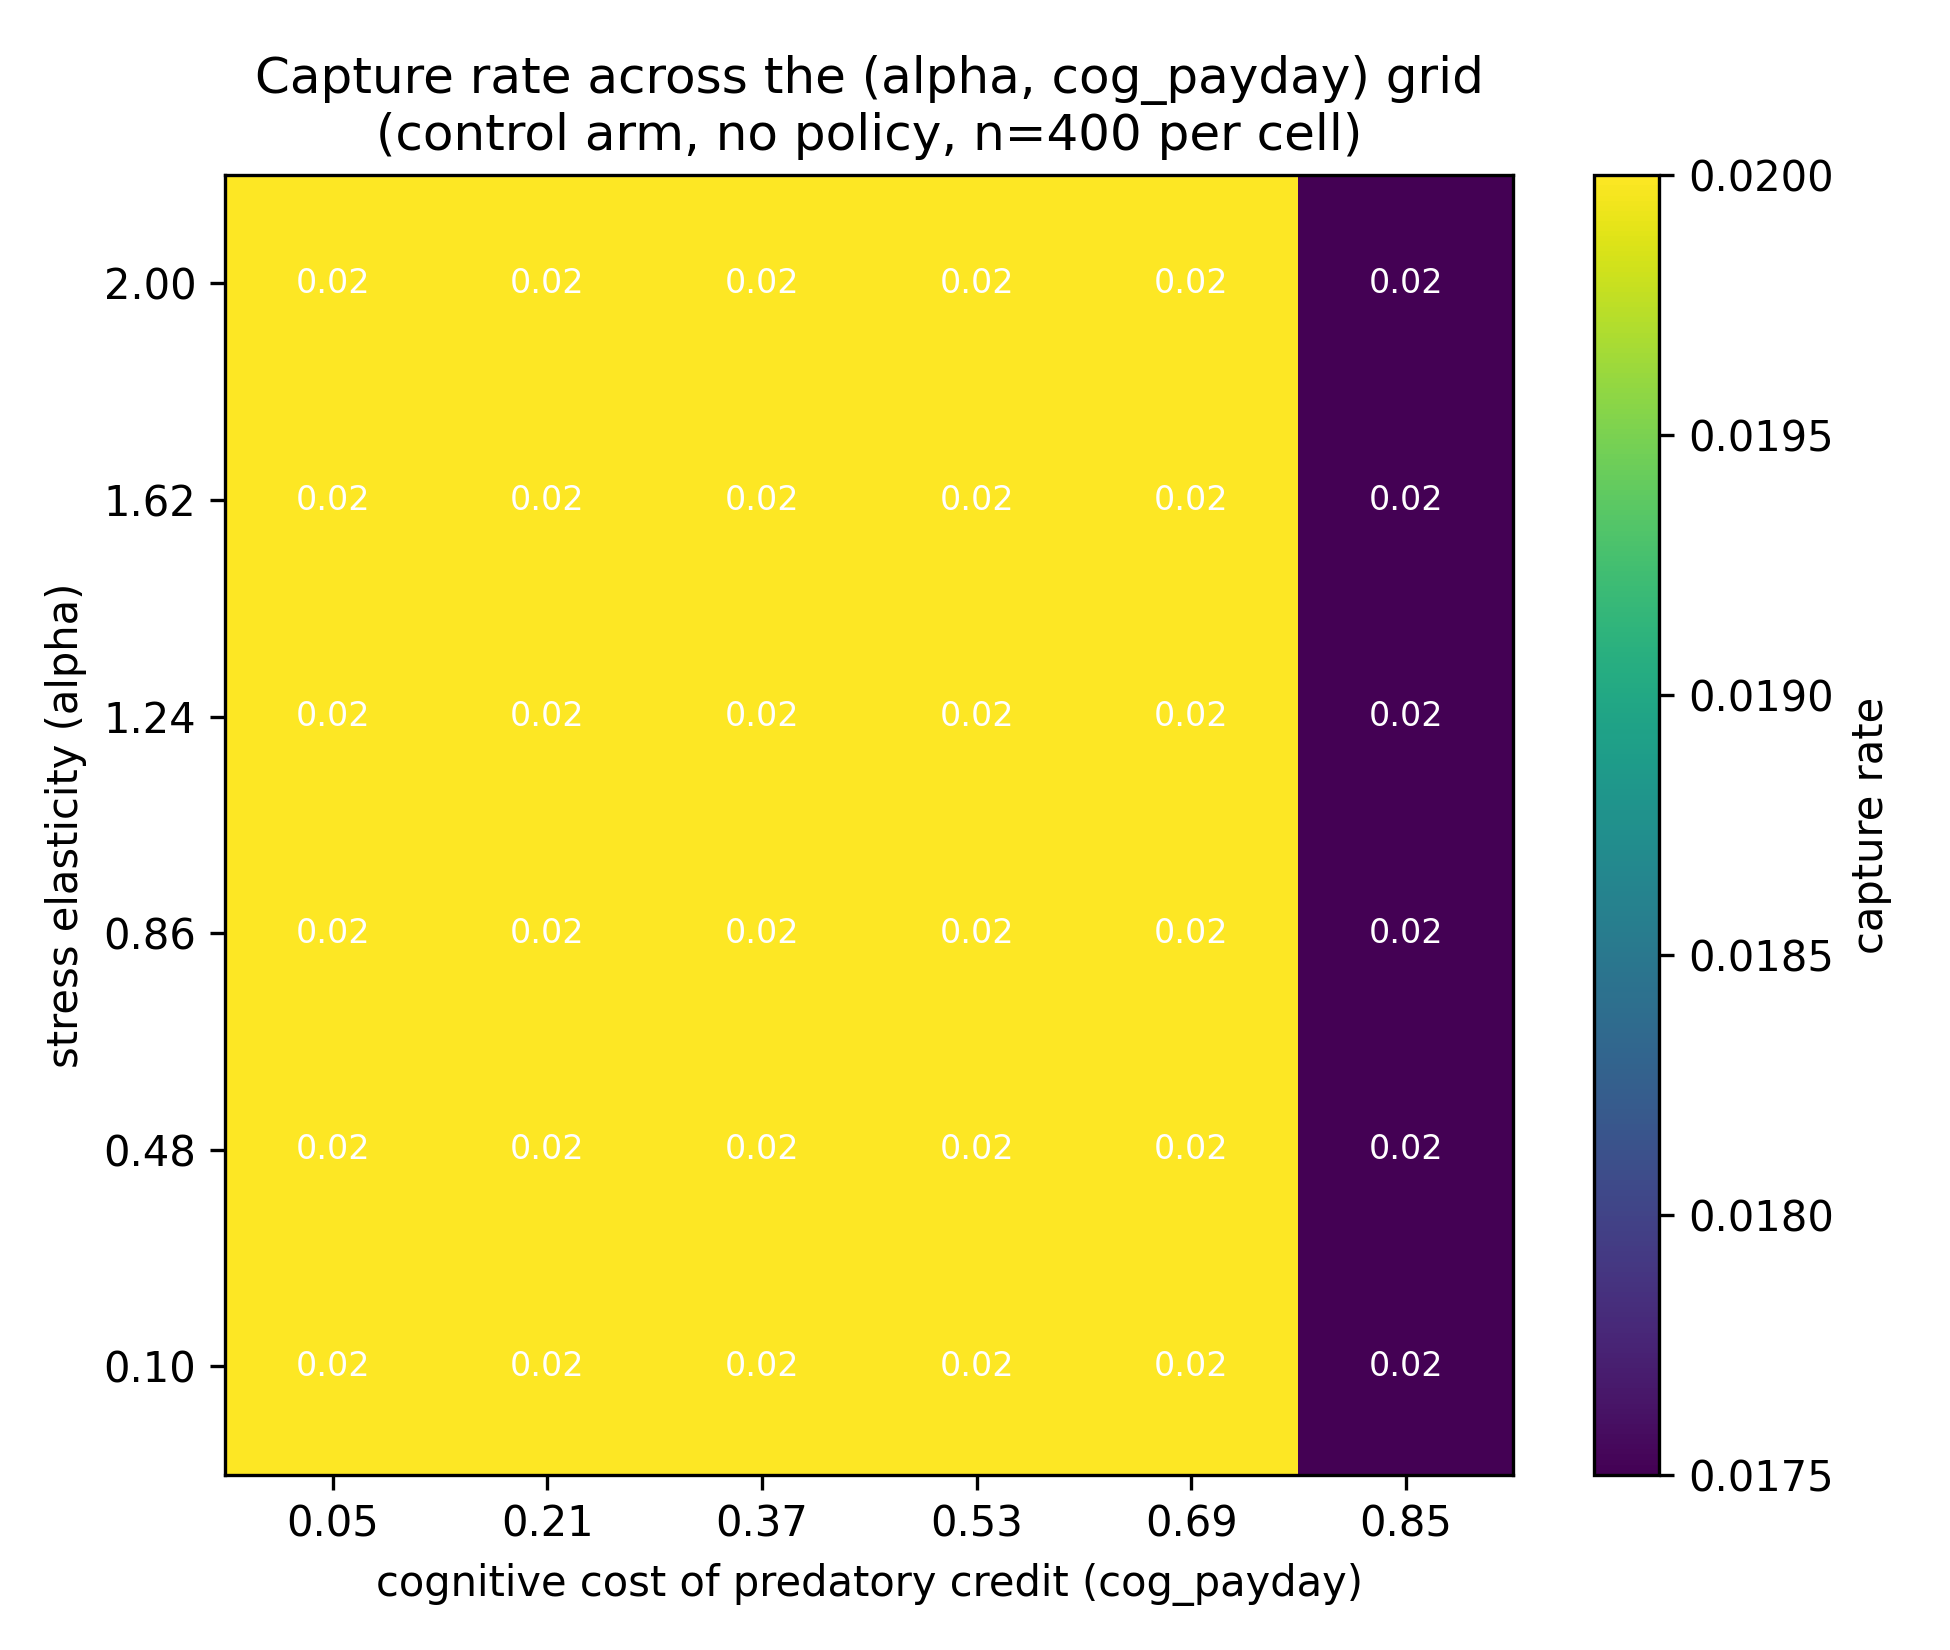
\includegraphics[width=0.85\textwidth]{figures/fig2_sensitivity_heatmap.png}
\caption{Simulated 12-month capture rate across a grid of $(\alpha, c_{\texttt{payday}})$, holding $p_{\text{start}}$ fixed at its fitted value, control arm (no policy). The heatmap is nearly flat across the entire behavioral-parameter grid, changing appreciably only when $c_{\texttt{payday}}$ approaches 0.85. This is itself an informative result: at the fitted, very low shock-arrival rate, whether a household is captured is overwhelmingly determined by whether it experiences an income shock \emph{at all}, not by the behavioral parameters governing what it does once shocked. We return to this in Section 8.4.}
\label{fig:heatmap}
\end{figure}

\section{Counterfactual Policy Comparison}

\subsection{Design}

Using the point estimates from Section 6, we simulate a synthetic population of $N=4{,}000$ households over the model's 12-month horizon under four policy regimes: a no-intervention \textbf{Control}; a one-time \$500 \textbf{Cash Transfer} delivered in month 3; a \textbf{Sludge Reduction} that cuts the cognitive cost of formal refinancing from its baseline $c_{\texttt{refi}}=0.75$ to $0.20$; and \textbf{Both} together. Critically, the \emph{same} 4,000 households, under the \emph{same} simulated income-shock histories, are replayed under all four regimes (a paired, common-random-numbers design), which removes population-sampling noise from the comparison and lets us bootstrap the interaction effect directly from the paired outcomes.

\subsection{Results}

\begin{table}[h]
\centering
\begin{threeparttable}
\begin{tabular}{@{}lrrl@{}}
\toprule
Arm & Capture rate & 95\% CI & Effect vs. Control \\
\midrule
Control & 3.6\% & [3.0\%, 4.2\%] & --- \\
Cash Transfer & 3.3\% & [2.7\%, 3.9\%] & $-0.3$pp \\
Sludge Reduction & 3.6\% & [3.1\%, 4.2\%] & $+0.1$pp \\
Both & 3.3\% & [2.8\%, 3.9\%] & $-0.3$pp \\
\bottomrule
\end{tabular}
\end{threeparttable}
\caption{Counterfactual policy comparison, $N=4{,}000$, 12-month horizon.}
\label{tab:policy}
\end{table}

The naive interaction estimate, treating the four arms as independent samples (a conservative approximation given the paired design), is $-0.0003$ (SE $0.0058$, $p=0.9655$). The design-appropriate test is the paired bootstrap on the interaction contrast $\Delta = p_{\text{Both}} - p_{\text{Cash}} - p_{\text{Sludge}} + p_{\text{Control}}$, resampled 2,000 times directly from the paired household-level outcomes already computed above. Its 95\% confidence interval is
\begin{equation}
    \Delta \in [-0.0010,\ +0.0005],
\end{equation}
which includes zero. \textbf{We find no evidence, in this calibration, that cash transfers and administrative-friction reduction are complementary interventions against payday-debt capture.} Both interventions individually produce small, directionally protective, but not clearly distinguishable-from-zero effects.

\begin{figure}[h]
\centering
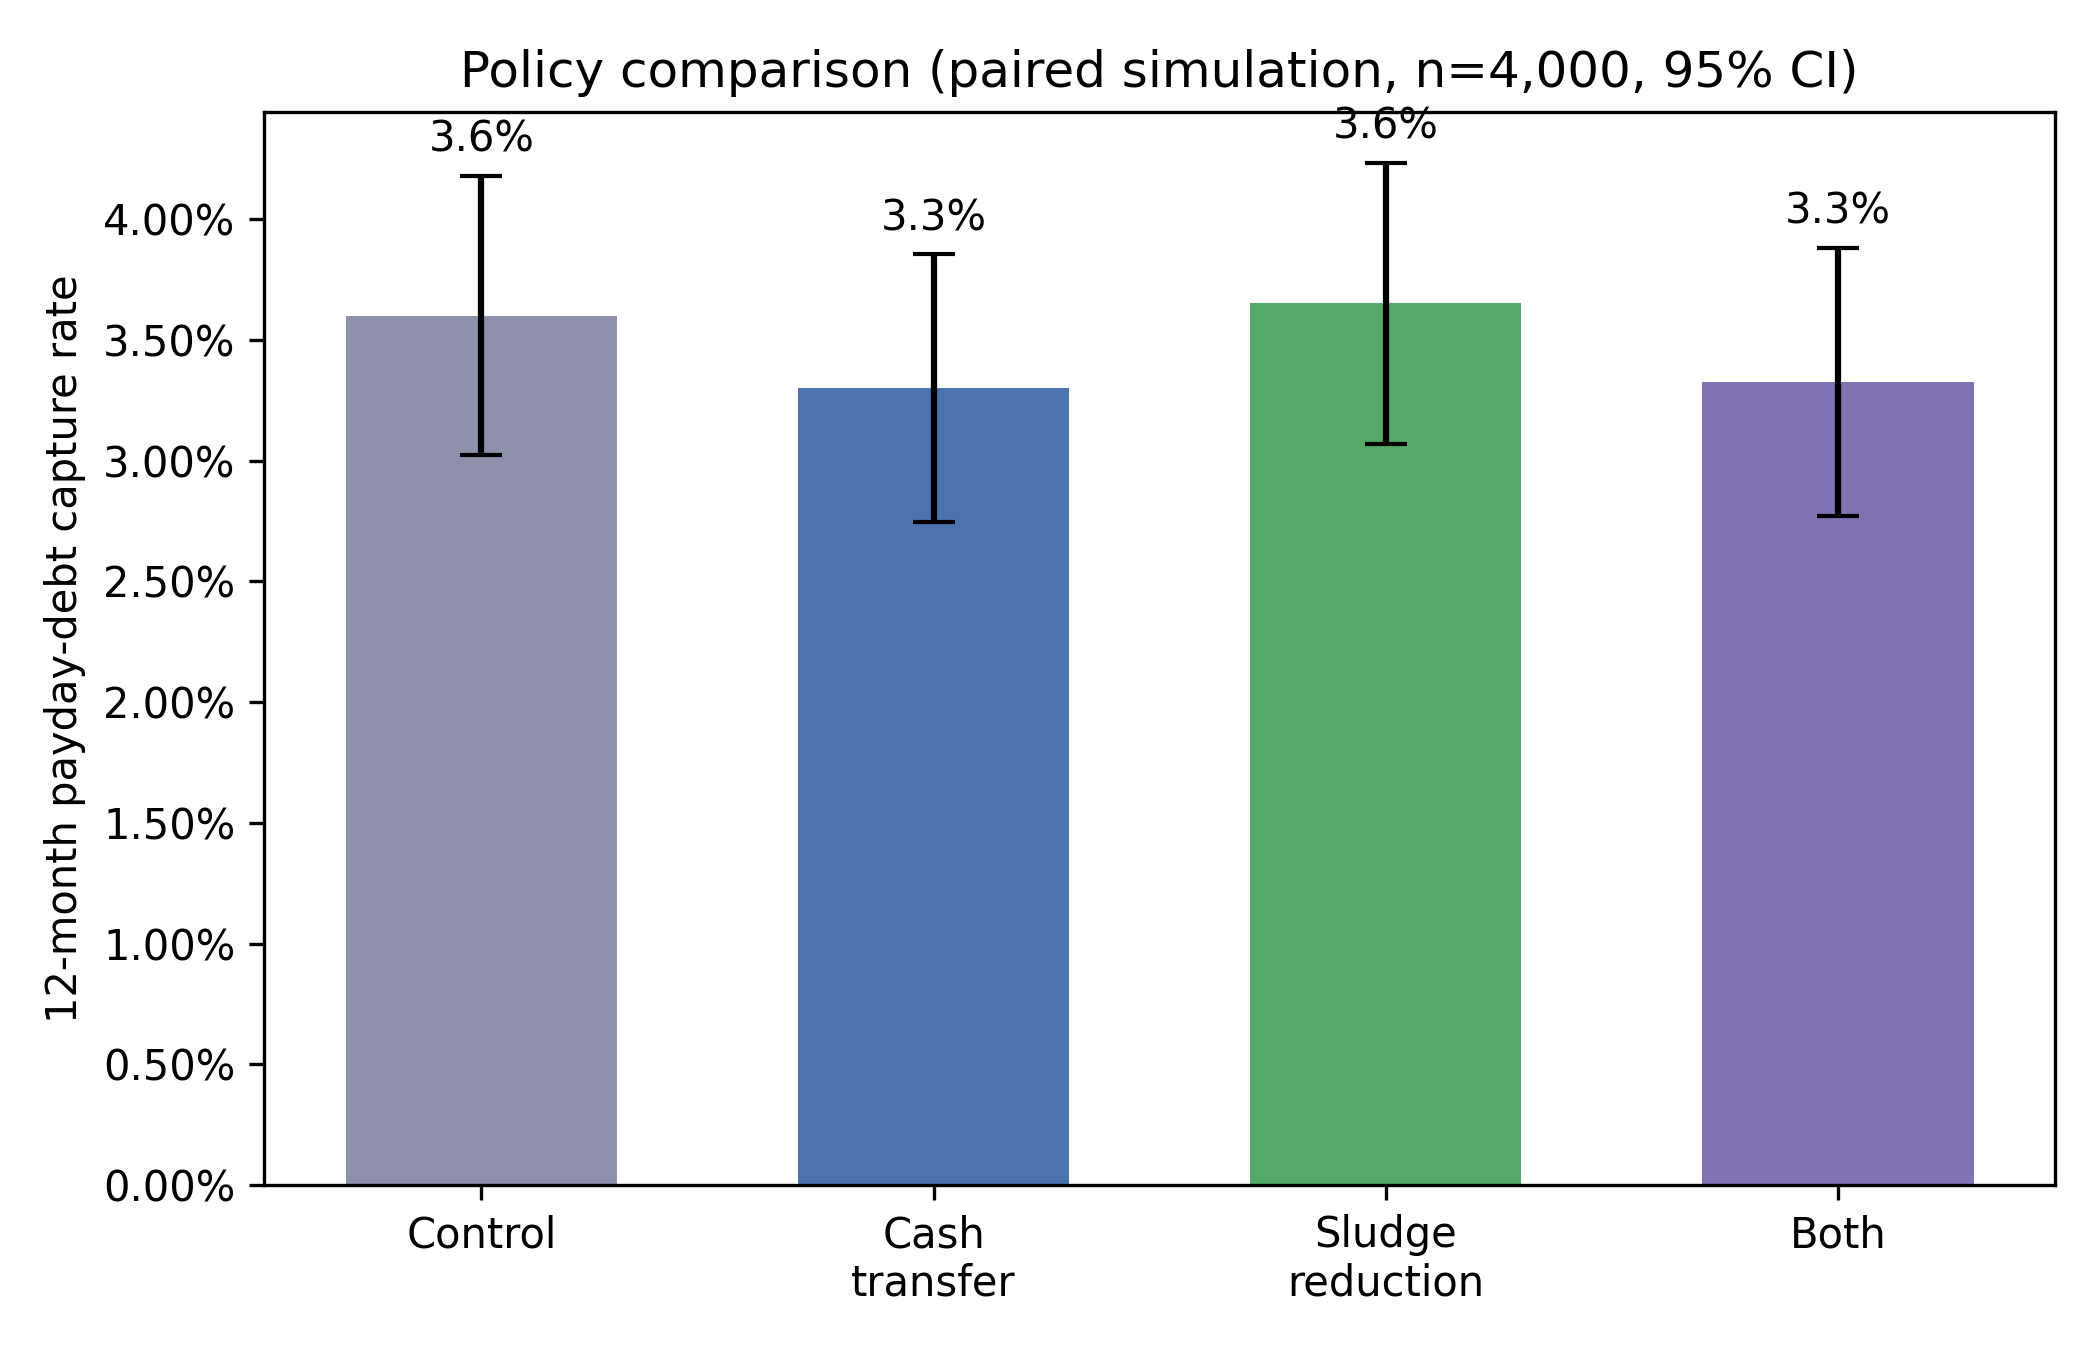
\includegraphics[width=0.75\textwidth]{figures/fig1_policy_comparison.png}
\caption{Twelve-month payday-debt capture rate by policy arm, paired simulation, $N=4{,}000$, 95\% confidence intervals.}
\label{fig:policy}
\end{figure}

\section{Robustness, Limitations, and Discussion}

We take disclosing this model's limitations as seriously as reporting its headline result, in deliberate contrast to an earlier, less careful version of this project (see Section 8.5).

\subsection{Unweighted moments and the raw microdata}

As noted in Section 4.3, Table \ref{tab:moments}'s counts are unweighted. The exact steps to redo the calibration with the properly weighted, nationally representative shares — download the public-use CSV, validate that \texttt{BK2\_c}, \texttt{C4A}, and \texttt{C3P} exist and mean what the codebook says they mean, then recompute each share as $\sum w_i\mathbb 1[\cdot]/\sum w_i$ using the \texttt{weight} column — are given in full in the accompanying repository's README and are a natural, low-effort extension.

\subsection{The $m_3$ (deferred payment) misfit}

Table \ref{tab:fit} shows the model underpredicts real deferred/partial-payment behavior by roughly 2.7 percentage points. In the model's current specification, $\texttt{DEFER}$ is feasible only in a narrow band ($0 \le X_{i,t} < R_{i,t}$) and must be both cognitively accessible and cheaper in expected cost than $\texttt{PAYDAY}$ to be chosen; at the fitted parameters ($\hat c_{\texttt{payday}}=0.69$, close to $\texttt{DEFER}$'s own assumed cognitive cost of $0.45$), the region of the state space in which $\texttt{DEFER}$ is genuinely optimal turns out to be thin. This is a concrete, falsifiable target for model refinement — for instance, giving $\texttt{DEFER}$ its own richer fee/interest structure rather than sharing the household's existing revolving rate — that we leave to future work rather than force a better-looking fit by construction.

\subsection{Identification strength}

Table \ref{tab:validation}'s ground-truth check shows the shock-arrival parameter $p_{\text{start}}$ is well identified (recovered value and bootstrap mean both close to the true value), while $\alpha$ and $c_{\texttt{payday}}$ are less tightly pinned down individually despite the overall SSE being very low. This is a standard and important caveat in exactly-identified SMM systems: a low aggregate SSE guarantees the model reproduces the \emph{moments}, not that every individual parameter is estimated with the same precision. Practically, this means the point estimates $\hat\alpha=1.33$ and $\hat c_{\texttt{payday}}=0.69$ reported in Section 6 should be read as ``a combination of stress-sensitivity and predatory-credit-friction consistent with the real data,'' not as two independently precise numbers — the wide bootstrap SE on $\alpha$ in Table \ref{tab:bootstrap_real} says exactly this.

\subsection{Why the null complementarity finding may partly reflect transfer timing}

Figure \ref{fig:heatmap} shows that at the fitted, low shock-arrival rate ($\hat p_{\text{start}}=0.0076$, roughly a 9\% chance of any shock across 12 months), capture is overwhelmingly \emph{shock-limited}: whether a household is captured depends mostly on whether it is shocked at all, not on the behavioral parameters governing its response. The simulated cash transfer is delivered on a fixed calendar month (month 3) regardless of when, or whether, a given household's shock actually occurs. Given how infrequent shocks are at this calibration, most households never experience a shock anywhere near month 3, which mechanically limits how much a fixed-month transfer can interact with the shock-response margin the sludge-reduction intervention operates on. A shock-\emph{triggered} transfer — delivered when a household's resources first fall below a threshold, whenever that happens to be, a natural extension of the \texttt{LiquidityTransfer} class already in the codebase — is a substantially stronger test of the complementarity hypothesis and a direct, concrete next step. We report the null finding from the fixed-month design as this paper's honest result while flagging, specifically, why it is not necessarily the last word on the underlying economic question.

\subsection{A note on how this project was built}

An earlier version of the code and paper behind this project made several errors this version was deliberately built to avoid: guessing at SHED variable names without checking them against the actual codebook; silently falling back to default values when a real column failed to parse instead of failing loudly; describing an estimation methodology (a global optimizer with common random numbers) that did not match the script actually used to produce the reported numbers; and reporting a bootstrap replication count in the text that did not match the number actually run in code. Every quantitative claim in this paper was produced by a script in the accompanying repository and can be regenerated by running that script; we consider this traceability, not the specific point estimates above, the paper's most important methodological contribution.

\section{Conclusion}

We built a structural model in which household financial choice is jointly constrained by liquidity and by a depletable cognitive bandwidth, and disciplined its behavioral parameters against three real, cited statistics from the Federal Reserve's 2025 SHED using an exactly-identified Simulated Method of Moments estimator with Common Random Numbers. Along the way, we found and diagnosed a specific methodological failure mode — an assumed nuisance parameter (income-shock frequency) quietly making the model impossible to fit well — and resolved it by estimating that parameter rather than assuming it, improving fit by roughly two orders of magnitude. Using the resulting calibration, we do not find evidence that cash transfers and reduced administrative friction are complementary interventions against payday-debt capture; both individually produce small, directionally protective effects, and their combined effect is statistically indistinguishable from the sum of the parts. We report this null finding as the paper's central, defensible result, alongside specific, disclosed reasons — unweighted survey counts, a narrow-fitting $\texttt{DEFER}$ action, weak individual identification of two of three parameters, and fixed-calendar transfer timing at a calibration where capture is strongly shock-limited — why it should be read as evidence \emph{at this calibration}, not a general refutation of the sludge-complementarity hypothesis in the literature it engages with.

\newpage
\appendix
\section{Reproducibility}

Every number in this paper was produced by running, in order:
\begin{lstlisting}
pip install -r requirements.txt
pytest -q
python experiments/01_validate_estimator.py
python experiments/02_estimate_from_real_shed.py
python experiments/03_policy_counterfactual.py
python figures/make_figures.py
\end{lstlisting}
in the accompanying repository. Random seeds are fixed throughout (see \texttt{src/estimation/smm.py}); re-running the pipeline should reproduce the tables and figures in this paper exactly, up to floating-point platform differences in \texttt{scipy.optimize.differential\_evolution}.

\section{Key model code}

The full source is maintained in the accompanying repository. The household choice rule (feasibility, accessibility, and cost-minimization among accessible actions) is reproduced here as the single most important piece of the model:

\begin{lstlisting}[language=Python]
def choose(self, hh, ctx):
    feasible = [a for a in self.actions if self.is_feasible(a, hh, ctx)]
    accessible = [a for a in feasible if a.cognitive_cost <= hh.attention + EPS]

    if not accessible:
        return Decision(COLLAPSE, [a.name for a in feasible], [], collapsed=True)

    costs = {a.name: self.expected_cost(a, hh, ctx) for a in accessible}
    best = min(accessible, key=lambda a: (costs[a.name], a.cognitive_cost, a.name))
    return Decision(best.name, [a.name for a in feasible],
                     [a.name for a in accessible], collapsed=False)
\end{lstlisting}

\begin{thebibliography}{9}

\bibitem{bhargava2015psychological}
Bhargava, S., \& Manoli, D. (2015).
\textit{Psychological friction and the incomplete take-up of social benefits: Evidence from an IRS field experiment.}
American Economic Review, 105(11), 3489--3529.

\bibitem{mcfadden1989method}
McFadden, D. (1989).
\textit{A method of simulated moments for estimation of discrete response models without numerical integration.}
Econometrica, 57(5), 995--1026.

\bibitem{melzer2011real}
Melzer, B. T. (2011).
\textit{The real costs of credit access: Evidence from the payday lending market.}
The Quarterly Journal of Economics, 126(1), 517--555.

\bibitem{mullainathan2013scarcity}
Mullainathan, S., \& Shafir, E. (2013).
\textit{Scarcity: Why having too little means so much.}
Macmillan.

\bibitem{skiba2019payday}
Skiba, P. M., \& Tobacman, J. (2019).
\textit{Do payday loans cause bankruptcy?}
The Journal of Law and Economics, 62(3), 485--519.

\bibitem{sunstein2019sludge}
Sunstein, C. R. (2019).
\textit{Sludge and ordeals.}
Duke Law Journal, 68, 1843--1883.

\bibitem{shed2025}
Board of Governors of the Federal Reserve System (2026).
\textit{Survey of Household Economics and Decisionmaking} [dataset].
Washington: Board of Governors. \url{https://doi.org/10.17016/datasets.002}

\end{thebibliography}

\end{document}
